\documentclass[11pt,a4paper]{article}
\usepackage[utf8]{inputenc}
\usepackage[T1]{fontenc}
\usepackage{lmodern}
\usepackage[brazil]{babel}
\usepackage[margin=1.8cm]{geometry}
\usepackage{amsmath,amssymb}
\usepackage{graphicx}
\usepackage{float}
\usepackage{needspace}
\usepackage{booktabs,longtable,array,multirow,makecell}
\usepackage{xcolor}
\usepackage{enumitem}
\usepackage{tikz}
\usetikzlibrary{positioning,arrows.meta,shapes.misc,calc,fit,backgrounds}
\usepackage[hidelinks]{hyperref}
\makeatletter\let\inputtab\@@input\makeatother  % \input primitivo: funciona dentro de tabelas
\usepackage{caption}
\captionsetup{font=small,labelfont=bf}

% ----------------------------- cores ---------------------------------
\definecolor{azul}{HTML}{2A78D6}
\definecolor{verde}{HTML}{1BAF7A}
\definecolor{amarelo}{HTML}{EDA100}
\definecolor{vermelho}{HTML}{B3261E}
\definecolor{cinza}{HTML}{6B6A64}
\definecolor{corpy}{HTML}{2A78D6}   % Python
\definecolor{corampl}{HTML}{C2410C} % AMPL
\definecolor{corcpp}{HTML}{7C3AED}  % C++

% ------------------------ marcador de atenção -------------------------
\newcommand{\lpy}{\tikz[baseline=(c.base)]\node[rounded corners=1.5pt,fill=corpy,text=white,
  font=\scriptsize\bfseries\sffamily,inner sep=1.4pt](c){Python};}
\newcommand{\lam}{\tikz[baseline=(c.base)]\node[rounded corners=1.5pt,fill=corampl,text=white,
  font=\scriptsize\bfseries\sffamily,inner sep=1.4pt](c){AMPL};}
\newcommand{\lcpp}{\tikz[baseline=(c.base)]\node[rounded corners=1.5pt,fill=corcpp,text=white,
  font=\scriptsize\bfseries\sffamily,inner sep=1.4pt](c){C++};}
% \atp{n}: pergunta PRINCIPAL (vermelho); \ats{n}: pergunta secundária (cinza)
\newcommand{\atp}[1]{\tikz[baseline=(c.base)]\node[circle,fill=vermelho,text=white,
  font=\scriptsize\bfseries,inner sep=0.6pt,minimum size=4.6mm](c){P#1};}
\newcommand{\ats}[1]{\tikz[baseline=(c.base)]\node[circle,fill=cinza!45,text=white,
  font=\scriptsize\bfseries,inner sep=0.6pt,minimum size=4.6mm](c){S#1};}
\newcommand{\at}[1]{\tikz[baseline=(c.base)]\node[circle,fill=vermelho,text=white,
  font=\scriptsize\bfseries,inner sep=0.6pt,minimum size=4.6mm](c){A#1};}

% --------------------------- estilos TikZ -----------------------------
\tikzset{
  base/.style={rectangle, rounded corners=2pt, draw=black!65, align=center,
               font=\small, inner sep=3pt, minimum height=7mm},
  proc/.style={base, fill=white, text width=#1}, proc/.default=5.4cm,
  ini/.style={base, rounded corners=9pt, fill=azul!12, draw=azul, text width=#1},
  ini/.default=5.4cm,
  dec/.style={chamfered rectangle, chamfered rectangle xsep=2mm, draw=amarelo!80!black,
              fill=amarelo!18, align=center, font=\small, text width=#1, inner sep=2pt,
              minimum height=7mm}, dec/.default=5.0cm,
  ok/.style={base, fill=verde!15, draw=verde!80!black, text width=#1}, ok/.default=3.0cm,
  alt/.style={base, dashed, draw=cinza, text=cinza, fill=white, text width=#1},
  alt/.default=3.0cm,
  ruim/.style={base, fill=vermelho!10, draw=vermelho, text width=#1}, ruim/.default=3.0cm,
  atens/.style={circle, fill=cinza!45, text=white, font=\scriptsize\bfseries,
               inner sep=0.6pt, minimum size=4.8mm},
  aten/.style={circle, fill=vermelho, text=white, font=\scriptsize\bfseries,
               inner sep=0.6pt, minimum size=4.8mm},
  seta/.style={-{Stealth[length=2.2mm]}, thick, draw=black!70},
  fina/.style={-{Stealth[length=1.8mm]}, draw=cinza, dashed},
  rot/.style={font=\scriptsize, text=black!75, fill=white, inner sep=1pt},
  grupo/.style={draw=cinza, dashed, rounded corners=4pt, inner sep=3mm},
  tag/.style={rounded corners=1.5pt, font=\tiny\bfseries\sffamily, text=white, inner sep=1.4pt,
              anchor=south west, xshift=1.5mm, yshift=0.3mm},
  py/.style={tag, fill=corpy}, am/.style={tag, fill=corampl}, cpp/.style={tag, fill=corcpp},
  faixa/.style={rounded corners=2pt, font=\small\sffamily, text width=#1, align=center,
                inner sep=3pt, text=white}, faixa/.default=12cm,
}

\title{\textbf{Fluxo do projeto 2BPPC}\\[2pt]
\large Empacotamento bidimensional em contêineres com conflitos\\
\normalsize Método exato (AMPL) $\times$ metaheurística (RKO/BRKGA)}
\author{Arthur Santos de Oliveira --- Pesquisa Operacional, UNIFESP--ICT}
\date{Material de estudo e de conversa com o professor --- novembro de 2026}

\begin{document}
\maketitle
\tableofcontents

% =====================================================================
\section{Como ler este documento}
% =====================================================================
Cada fluxograma mostra \emph{o que o código faz, na ordem em que faz}. As escolhas de projeto
aparecem ao lado do passo em que atuam:

\begin{center}
\begin{tikzpicture}[node distance=3mm and 4mm]
  \node[proc=2.6cm] (a) {passo do algoritmo};
  \node[dec=2.6cm, right=of a] (b) {decisão (sim/não)};
  \node[ok=2.6cm, right=of b] (c) {opção \textbf{escolhida} \checkmark};
  \node[alt=2.6cm, right=of c] (d) {alternativa implementada, não usada};
  \node[ini=2.6cm, below=of a] (e) {início / fim};
  \node[ruim=2.6cm, right=of e] (f) {resultado negativo};
  \node[aten, right=8mm of f] (g) {P1};
  \node[atens, right=1mm of g] (g2) {S1};
  \node[right=1mm of g2, font=\small, text width=5.2cm, align=left]
       {pergunta para o professor: \textbf{principal} (vermelho) ou secundária (cinza) (Seção~\ref{sec:atencao})};
\end{tikzpicture}
\end{center}
\noindent\textbf{Linguagem de cada parte:} \lpy\ Python 3.10 (dados, pré-processamento, verificador,
experimentos, tabelas) \quad \lam\ AMPL + solver HiGHS (método exato) \quad \lcpp\ C++20, g++ 11.4 +
OpenMP (decodificador e RKO). Cada fluxograma tem uma faixa no topo com a linguagem dele; caixas de outra
linguagem levam a etiqueta correspondente.

Há \textbf{4 perguntas principais} (\atp{1}--\atp{4}, em vermelho), que são as que importa levar ao
professor, e 7 secundárias (\ats{1}--\ats{7}, em cinza), que podem ficar para depois. A numeração é a mesma de
\texttt{docs/duvidas\_professor.md}. A Seção~\ref{sec:atencao} traz cada pergunta com contexto, números e espaço
para anotar a resposta.

% =====================================================================
\section{Visão geral}
% =====================================================================
\begin{figure}[H]
\centering
\begin{tikzpicture}[node distance=8mm and 6mm]
  \node[ini=3.6cm] (zip) {Instâncias do zip \texttt{2bppc/}\\(52 arquivos, $n=25$)};
  \node[proc=3.8cm, right=of zip] (fix) {Correção dos dados:\\01 reconstruída; 53--64 geradas};
  \node[proc=4.4cm, right=of fix] (pre) {Leitor + pré-processamento:\\arestas D (12), cliques (13), LB (14), UB guloso};
  \node[atens] at (fix.north east) {S6};
  \node[tag, fill=cinza] at (zip.north west) {arquivos texto};
  \node[py] at (fix.north west) {Python};
  \node[py] at (pre.north west) {Python};

  \node[proc=5.6cm, below=12mm of fix.south west, anchor=north east, xshift=10mm] (ex)
       {\textbf{MÉTODO EXATO} (AMPL + HiGHS)\\ mestre PLI + laço de cortes + 2D-OPP exato\\
        \scriptsize\texttt{ampl/bppc.mod}, \texttt{bppc.run} --- Figs.~\ref{fig:laco} e \ref{fig:testa}};
  \node[proc=5.6cm, below=12mm of pre.south east, anchor=north east] (mh)
       {\textbf{METAHEURÍSTICA} (RKO v2.0.1 + decodificador do projeto)\\ BRKGA sozinho ou RKO completo\\
        \scriptsize\texttt{meta/src/} --- Figs.~\ref{fig:dec} e \ref{fig:rko}};
  \node[aten] at (ex.north east) {P4};
  \node[aten] at (mh.north east) {P2};
  \node[am] (tex) at (ex.north west) {AMPL};
  \node[py, anchor=south west, xshift=0.8mm, yshift=0mm] at (tex.south east) {Python: .dat e lote};
  \node[cpp] (tmh) at (mh.north west) {C++};
  \node[py, anchor=south west, xshift=0.8mm, yshift=0mm] at (tmh.south east) {Python: lote};

  \node[proc=5.6cm, below=8mm of ex] (aud) {Auditoria dos cortes com outro método exato\\(CP-SAT, \texttt{NoOverlap2D})};
  \node[proc=5.6cm, below=8mm of mh] (ver) {\textbf{Verificador independente}\\ sobreposição, limites, conflitos, todos alocados};
  \node[ini=9cm, below=8mm of $(aud.south)!0.5!(ver.south)$] (res)
       {Tabelas das Etapas 5 e 6, performance profile, boxplot, desenhos das caixas};

  \node[py] at (aud.north west) {Python + OR-Tools};
  \node[py] at (ver.north west) {Python};
  \node[py] at (res.north west) {Python};
  \draw[seta] (zip) -- (fix);  \draw[seta] (fix) -- (pre);
  \draw[seta] (pre.south) -- ++(0,-5mm) -| (ex.north);
  \draw[seta] (pre.south) -- ++(0,-5mm) -| (mh.north);
  \draw[seta] (ex) -- (aud);
  \draw[seta] (ex.east) -- ++(4mm,0) |- (ver.west);
  \draw[seta] (mh) -- (ver);
  \draw[seta] (aud.south) -- ++(0,-2mm) -| ($(res.north)+(-2cm,0)$);
  \draw[seta] (ver.south) -- ++(0,-2mm) -| ($(res.north)+(2cm,0)$);
\end{tikzpicture}
\caption{Fluxo geral. Os dois métodos usam a mesma leitura e o mesmo pré-processamento, e
toda solução, venha de onde vier, passa pelo mesmo verificador.}
\label{fig:geral}
\end{figure}

\paragraph{Mapa dos arquivos (para estudar).}
\begin{center}\small
\begin{tabular}{@{}p{5.4cm}lp{9.2cm}@{}}
\toprule
Arquivo & Ling. & O que faz \\ \midrule
\texttt{src/bppc/instance.py} & \lpy & lê as instâncias (itens, $W$, $H$, matriz de conflitos) \\
\texttt{src/bppc/preprocess.py} & \lpy & arestas por dimensão, cliques, LB, UB guloso, ordem dos itens \\
\texttt{src/bppc/geometry.py} & \lpy & Maximal Rectangles em Python (só para o UB do exato) \\
\texttt{src/bppc/solution.py} & \lpy & formato de solução e \textbf{verificador independente} \\
\texttt{src/bppc/opp\_cpsat.py} & \lpy & 2D-OPP em CP-SAT (auditoria dos cortes) \\
\texttt{src/bppc/plot.py} & \lpy & desenho das caixas \\
\texttt{ampl/gerar\_dat.py} & \lpy & gera o \texttt{.dat} pré-processado \\
\texttt{ampl/bppc.mod} & \lam & modelo mestre + 2D-OPP (dois \texttt{problem}) \\
\texttt{ampl/bppc.run}, \texttt{testa\_grupo.run} & \lam & laço de cortes; teste ``o grupo cabe?'' \\
\texttt{ampl/rodar\_ampl.py} & \lpy & roda as 64 instâncias e confere as soluções \\
\texttt{meta/src/Problem\_2BPPC.h} & \lcpp & \textbf{decodificador} (a parte do RKO que escrevemos) \\
\texttt{meta/RKO\_Cpp\_v2.0/} & \lcpp & RKO original (metaheurísticas), sem modificação \\
\texttt{meta/src/rko\_bppc.cpp} & \lcpp & \texttt{main} adaptado do RKO \\
\texttt{meta/config/*.conf} & texto & quais metaheurísticas rodam (só BRKGA ou as 10) \\
\texttt{meta/experimentos.py}, \texttt{analisar.py} & \lpy & execuções em lote e resumo contra o ótimo \\
\texttt{scripts/} & \lpy & instâncias geradas, auditoria, tabelas, gráficos, este documento \\
\texttt{docs/decisoes.md}, \texttt{duvidas\_professor.md} & texto & decisões (com motivo) e perguntas \\
\bottomrule
\end{tabular}
\end{center}

% =====================================================================
\section{Dados e pré-processamento}
% =====================================================================
\begin{itemize}[leftmargin=*,itemsep=2pt]
\item O zip tem só \textbf{52 arquivos}. As 53--64 foram \textbf{geradas} copiando a original
  indicada no artigo-base (53$\leftarrow$21, 54$\leftarrow$38, \dots) com caixa $60\times60$. A regra
  foi conferida nas cópias que existem: 50$\equiv$18, 51$\equiv$35 e 52$\equiv$04. \ats{6}
\item O arquivo \texttt{2kdc01} é uma \textbf{cópia exata da 02}. A 01 foi reconstruída como
  ``49 com caixa $30\times30$''. Os arquivos originais não foram alterados. \ats{6}
\item Pré-processamento (igual para os dois métodos):
  \begin{itemize}[itemsep=0pt]
  \item \textbf{arestas D} (regra 12): se $w_i+w_j>W$ e $h_i+h_j>H$, os itens nunca cabem juntos
    $\Rightarrow$ nova aresta de conflito;
  \item \textbf{cliques maximais} ($\ge3$ itens) do grafo estendido: cada clique exige caixas distintas;
  \item \textbf{LB} $=\max(\lceil\text{área}/WH\rceil,\ \text{maior clique})$;
  \item \textbf{UB guloso}: melhor de 204 ordens $\times$ \{FF, BF\} $\times$ \{BSSF, BL\}.
    Ele já acha o ótimo em 55 das 64 instâncias; em 26, empata com o LB e prova o ótimo sozinho.
  \end{itemize}
\end{itemize}

% =====================================================================
\section{Método exato (Etapa 5)}
% =====================================================================
\subsection{O modelo, em uma tabela}
\begin{center}\small
\begin{tabular}{@{}lp{12.4cm}@{}}
\toprule
(1) & $\min \sum_k \beta_k$ (nº de caixas) \\
(2) & área: $\sum_i w_ih_i\alpha_{ik}\le WH\beta_k$ \\
(3) & cada item em exatamente uma caixa \\
(4)+(12) & conflito: $\alpha_{ik}+\alpha_{jk}\le1$ para arestas originais e arestas D \\
(5) & \textbf{geometria}: $\sum_{i\in S}\alpha_{ik}\le|S|-1$ para grupos $S$ que não cabem ---
      \emph{gerada sob demanda pelo laço} \\
(8)--(10) & quebra de simetria: item 1 na caixa 1; caixas consecutivas; item $i$ numa das $i$
      primeiras caixas ($i\le n/2$) \\
(11) & pilha de itens largos $\le H\beta_k$; fileira de itens altos $\le W\beta_k$ \\
(13), (14) & cliques $\sum_{i\in C}\alpha_{ik}\le\beta_k$; $\sum_k\beta_k\ge$ LB \\
\midrule
\multicolumn{2}{@{}p{15.6cm}@{}}{\textbf{Decisões extras:} $K=\{1..\text{UB}\}$ em vez de $\{1..n\}$
(o modelo encolhe de 650 para $\le$ 525 variáveis); itens renumerados por grau de conflito
decrescente (ordem ``Oc'' do artigo-base), para que (8) e (10) fixem primeiro os itens mais difíceis.} \\
\bottomrule
\end{tabular}
\end{center}

\subsection{O laço de cortes}
\begin{figure}[H]
\centering
\begin{tikzpicture}[node distance=5.5mm and 7mm]
  \node[ini] (i0) {Início: nenhum corte (5), cache vazio};
  \node[faixa=13cm, fill=corampl, above=9mm of i0] (fx) {\textbf{AMPL} --- \texttt{ampl/bppc.run}
        (laço) e \texttt{ampl/bppc.mod} (modelo); solver HiGHS};
  \node[proc=3.4cm, left=10mm of i0] (dat) {Entrada: \texttt{.dat} pré-processado\\
        \scriptsize\texttt{ampl/gerar\_dat.py}};
  \node[py] at (dat.north west) {Python};
  \draw[seta] (dat) -- (i0);
  \node[proc, below=of i0] (m) {Resolve o \textbf{MESTRE} com HiGHS\\
        \scriptsize (1)--(4), (8)--(14) + cortes (5) já conhecidos};
  \node[dec, below=of m] (t) {Estourou o tempo (3600\,s)?};
  \node[proc, below=of t] (k) {Para cada caixa usada $k$:\\ $P\leftarrow$ itens que o mestre pôs em $k$};
  \node[dec, below=of k] (c) {$P$ cabe numa caixa? \\ \scriptsize (teste exato, Fig.~\ref{fig:testa})};
  \node[proc, below=of c] (red) {\textbf{Reduz} $P$: tenta tirar cada item, do menor para o maior; tira se
        o grupo \emph{continua} não cabendo};
  \node[proc, below=of red] (cut) {Acrescenta o corte (5) para o $P$ reduzido \textbf{em todas as caixas}};
  \node[dec, below=of cut] (novo) {Algum corte novo nesta rodada?};
  \node[ini, below=of novo] (fim) {\textbf{ÓTIMO}: o mestre é ótimo e todas as caixas cabem.\\
        Reconstrói coordenadas inteiras e grava a solução};
  \node[ruim=3.4cm, right=of t] (tl) {Reporta LB e UB guloso\\ \scriptsize (não aconteceu)};
  \node[ok=3.4cm, right=of c] (prox) {cabe: guarda no cache,\\ vai para a próxima caixa};
  \node[proc=3.4cm, right=of fim] (ver) {Verificador +\\ auditoria CP-SAT};

  \draw[seta] (i0) -- (m);  \draw[seta] (m) -- (t);
  \draw[seta] (t) -- node[rot]{sim} (tl);
  \draw[seta] (t) -- node[rot,right]{não} (k);
  \draw[seta] (k) -- (c);
  \draw[seta] (c) -- node[rot]{sim} (prox);
  \draw[seta] (c) -- node[rot,right]{não} (red);
  \draw[seta] (red) -- (cut);  \draw[seta] (cut) -- (novo);
  \draw[seta] (prox.south) |- (novo.east) node[rot, pos=0.25, right]{(após a última caixa)};
  \draw[seta] (novo.west) -- ++(-9mm,0) node[rot, above, pos=0.5]{sim} |- (m.west);
  \draw[seta] (novo) -- node[rot,right]{não} (fim);
  \draw[seta] (fim) -- (ver);
  \node[py] at (ver.north west) {Python};
  \node[aten] at (i0.north east) {P4};
\end{tikzpicture}
\caption{Laço de cortes (\texttt{ampl/bppc.run}). O AMPL não tem \emph{callbacks}, então o mestre
é resolvido várias vezes, ganhando um corte a cada grupo que não cabe. O mestre sem todos os cortes é uma
relaxação, logo seu valor é sempre um limitante inferior válido.}
\label{fig:laco}
\end{figure}

\begin{figure}[H]
\centering
\begin{tikzpicture}[node distance=3.5mm and 8mm]
  \node[ini=5cm] (p) {Grupo $P$ (itens de uma caixa)};
  \node[faixa=11cm, fill=corampl, above=6mm of p] {\textbf{AMPL} --- \texttt{ampl/testa\_grupo.run}
        (chamado pelo laço); 2D-OPP em \texttt{ampl/bppc.mod}; solver HiGHS};
  \node[dec, below=of p] (d1) {$|P|\le1$ ou $P$ no cache de ``cabe''?};
  \node[dec, below=of d1] (d2) {$P$ no cache de ``não cabe''?};
  \node[dec, below=of d2] (d3) {Área de $P$ $> WH$?};
  \node[dec, below=of d3] (d4) {Pilha de largos $>H$ ou fileira de altos $>W$?};
  \node[proc, below=of d4] (opp) {\textbf{2D-OPP exato} (PLI disjuntivo, HiGHS):\\
     \scriptsize $x_i\le W-w_i$, $y_i\le H-h_i$; para cada par: esquerda/direita/abaixo/acima;\\
     \scriptsize relações impossíveis fixadas em 0; maior item no quadrante inferior esquerdo};
  \node[dec, below=of opp] (r) {Resultado do solver};
  \node[ok, right=of d1] (s1) {\textbf{cabe}};
  \node[ruim, right=of d2] (n2) {\textbf{não cabe}};
  \node[ruim, right=of d3] (n3) {\textbf{não cabe}};
  \node[ruim, right=of d4] (n4) {\textbf{não cabe}};
  \node[ruim=2.8cm, below=6mm of r] (rn) {inviável: \textbf{não cabe} (cache)};
  \node[ok=2.8cm, left=4mm of rn] (rs) {viável: \textbf{cabe} (cache)};
  \node[alt=2.8cm, right=4mm of rn] (rt) {limite de tempo: desconhecido};
  \draw[seta] (p) -- (d1);
  \draw[seta] (d1) -- node[rot]{sim} (s1);  \draw[seta] (d1) -- node[rot]{não} (d2);
  \draw[seta] (d2) -- node[rot]{sim} (n2);  \draw[seta] (d2) -- node[rot]{não} (d3);
  \draw[seta] (d3) -- node[rot]{sim} (n3);  \draw[seta] (d3) -- node[rot]{não} (d4);
  \draw[seta] (d4) -- node[rot]{sim} (n4);  \draw[seta] (d4) -- node[rot]{não} (opp);
  \draw[seta] (opp) -- (r);
  \draw[seta] (r) -- (rn); \draw[seta] (r.south west) -- (rs.north); \draw[seta] (r.south east) -- (rt.north);
\end{tikzpicture}
\caption{Teste ``o grupo $P$ cabe numa caixa?'' (\texttt{ampl/testa\_grupo.run}). Do mais barato ao
mais caro. \textbf{Toda resposta é exata}: nenhum teste heurístico é usado aqui. O cache identifica
cada grupo pelo número $\sum_{i\in P}2^{i-1}$.}
\label{fig:testa}
\end{figure}

\paragraph{Como sabemos que os ótimos estão certos.}
(i) Toda solução do AMPL passou pelo verificador independente. (ii) Cada um dos 780 cortes foi
reconferido com outro método exato (CP-SAT): \textbf{todos os grupos proibidos realmente não cabem},
e todos são mínimos (tirando qualquer item, o grupo passa a caber).

% =====================================================================
\section{Metaheurística}
% =====================================================================
\subsection{O decodificador (a parte que escrevemos)}
As metaheurísticas do RKO só manipulam vetores de números em $[0,1)$. O decodificador transforma um
vetor numa solução e devolve uma nota (menor é melhor). Ele é a única parte que conhece o problema.
\textbf{Toda solução gerada é viável por construção.}

\begin{figure}[H]
\centering
\begin{tikzpicture}[node distance=5mm and 5mm]
  \node[ini=4.8cm] (r) {Vetor de chaves $r\in[0,1)^{n}$, $n=25$};
  \node[faixa=13cm, fill=corcpp, above=6mm of r, xshift=3.4cm] {\textbf{C++20} --- \texttt{meta/src/Problem\_2BPPC.h}
        (funções \texttt{Decodifica} e \texttt{Decoder}), compilado junto com o RKO};
  \node[proc=4.8cm, below=of r] (ord) {Ordena os itens pela chave\\(menor chave entra primeiro)};
  \node[proc=4.8cm, below=of ord] (prox) {Pega o próximo item $i$ da ordem};
  \node[proc=4.8cm, below=of prox] (cx) {Percorre as caixas abertas $k=1,2,\dots$};
  \node[dec=4.6cm, below=of cx] (conf) {Algum item de $k$ conflita com $i$?\\
        \scriptsize máscara de bits: 1 operação AND};
  \node[dec=4.6cm, below=of conf] (area) {Sobra área livre $\ge w_ih_i$?};
  \node[dec=4.6cm, below=of area] (geo) {Existe posição livre para $i$?\\ \scriptsize Maximal Rectangles};
  \node[proc=4.8cm, below=11mm of geo] (esc) {Caixa candidata: aplica a\\ \textbf{regra de escolha}};
  \node[dec=4.6cm, below=8mm of esc] (serve) {Alguma caixa serviu?};
  \node[proc=4.8cm, below=of serve] (coloca) {Coloca $i$ e recorta os retângulos livres};
  \node[dec=4.6cm, below=of coloca] (mais) {Ainda há itens?};
  \node[proc=4.8cm, below=of mais] (nota) {Calcula a \textbf{nota}};
  \node[dec=4.6cm, below=12mm of nota] (lb) {Nº de caixas $=$ LB?};
  \node[ini=4.8cm, below=10mm of lb] (ret) {Devolve a nota ao RKO};

  % alternativas à direita
  \node[ok=3.0cm, right=8mm of geo] (bl) {\textbf{Bottom-Left} \checkmark\\ \scriptsize mais baixo, depois mais à esquerda};
  \node[alt=2.6cm, right=3mm of bl] (bssf) {BSSF\\ \scriptsize menor sobra no lado curto};
  \node[ok=2.0cm, right=8mm of esc] (ff) {\textbf{FF} \checkmark\\ \scriptsize primeira que serve};
  \node[alt=2.0cm, right=3mm of ff] (bf) {BF\\ \scriptsize a mais cheia};
  \node[alt=2.5cm, right=3mm of bf] (ch) {chave ($2n$)\\ \scriptsize chave $n{+}i$ decide FF/BF};
  \node[proc=3.2cm, right=8mm of serve] (nova) {\textbf{não}: abre caixa nova;\\ $i$ em $(0,0)$};
  \node[ok=3.3cm, right=8mm of nota] (des) {\textbf{caixas + desempate} \checkmark\\
        \scriptsize $+$ área da caixa mais vazia$/WH$};
  \node[alt=2.4cm, right=3mm of des] (so) {só o nº de caixas};
  \node[proc=4.6cm, right=8mm of lb] (stop) {\textbf{sim}: ótimo provado. Avisa as metaheurísticas
        para pararem \scriptsize(\texttt{stop\_execution}, \texttt{MAXTIME}$=0$)};
  \node[proc=4.4cm, right=8mm of ord] (melhor) {\scriptsize Também guarda a melhor solução já vista e o
        instante em que apareceu (\texttt{tempo\_melhor})};

  \draw[seta] (r) -- (ord); \draw[seta] (ord) -- (prox); \draw[seta] (prox) -- (cx);
  \draw[seta] (cx) -- (conf);
  \draw[seta] (conf) -- node[rot,right]{não} (area);
  \draw[seta] (area) -- node[rot,right]{sim} (geo);
  \draw[seta] (geo) -- node[rot,right]{sim} (esc);
  \draw[seta] (esc) -- node[rot,right]{fim da busca} (serve);
  \draw[seta] (serve) -- node[rot,right]{sim} (coloca);
  \draw[seta] (serve) -- (nova);
  \draw[seta] (nova.south) |- (coloca.east);
  \draw[seta] (coloca) -- (mais);
  \draw[seta] (mais) -- node[rot,right]{não} (nota);
  \draw[seta] (nota) -- (lb);
  \draw[seta] (lb) -- node[rot,right]{não} (ret);
  \draw[seta] (lb) -- (stop);
  \draw[seta] (stop.south) |- (ret.east);
  % próxima caixa
  \coordinate (xl) at ($(conf.west)+(-8mm,0)$);
  \draw[seta] (conf.west) -- node[rot,above]{sim} (xl) |- (cx.west);
  \draw[thick, draw=black!70] (area.west) -- node[rot,above]{não} (area.west -| xl);
  \draw[thick, draw=black!70] (geo.west) -- node[rot,above]{não} (geo.west -| xl) -- (xl);
  \draw[thick, draw=black!70] (esc.west) -- node[rot,above]{BF/chave} (esc.west -| xl) -- (xl);
  \node[rot, rotate=90, anchor=south] at ($(geo.west -| xl)+(-1mm,0)$) {próxima caixa};
  % próximo item
  \coordinate (xl2) at ($(mais.west)+(-17mm,0)$);
  \draw[seta] (mais.west) -- node[rot,above]{sim} (xl2) |- (prox.west);
  % ligações das alternativas
  \draw[fina] (geo.east) -- (bl.west);
  \draw[fina] (esc.east) -- (ff.west);
  \draw[fina] (nota.east) -- (des.west);
  \draw[fina] (ord.east) -- (melhor.west);
  \node[atens] at (ord.north east) {S1};
  \node[aten] at (ff.north east) {P2};
  \node[atens] at (ch.north east) {S1};
  \node[atens] at (des.north east) {S2};
  \node[atens] at (stop.north east) {S7};
  \node[aten] at (lb.north east) {P3};
\end{tikzpicture}
\caption{Decodificador (\texttt{meta/src/Problem\_2BPPC.h}, funções \texttt{Decodifica} e
\texttt{Decoder}). Em verde, a variante escolhida; tracejadas, as alternativas implementadas
(parâmetros \texttt{--escolha}, \texttt{--posic}, \texttt{--aval}). Com FF, a busca pela caixa para na
primeira que serve; com BF, percorre todas e fica com a mais cheia. Exemplo de nota: 4{,}03 $=$ 4 caixas,
com a mais vazia 3\% cheia.}
\label{fig:dec}
\end{figure}

\paragraph{Por que o desempate importa.} Só com o nº de caixas, quase todas as ordens têm a mesma
nota (um ``platô''), e o BRKGA não sabe para onde ir. A área da caixa mais vazia diferencia soluções
com o mesmo nº de caixas: a que deixa uma caixa quase vazia está mais perto de eliminá-la.

\subsection{Testes rápidos das variantes (BRKGA)}
\paragraph{Como ler estas tabelas.} Uma \textbf{instância} é um arquivo de dados de entrada (ex.: \texttt{2kdc48}:
25 itens, caixa $50\times50$, lista de conflitos). Uma \textbf{execução} é rodar a metaheurística uma vez numa
instância, com uma \textbf{semente} (o número que inicia o gerador aleatório). A mesma semente faz sempre o mesmo
caminho de busca; sementes diferentes fazem buscas diferentes. Cada variante rodou 5 execuções (sementes 1--5) por
instância. As colunas:
\begin{itemize}[leftmargin=*,itemsep=0pt]
\item \textbf{\% ót.}: das execuções da variante (todas as instâncias juntas), quantas acharam o ótimo do método exato;
\item \textbf{\% 48}: o mesmo, mas \emph{só na instância 48}. Ela é a única em que as variantes se diferenciam; nas
  outras, quase todas acertam 100\%, e a média esconderia a diferença;
\item \textbf{T.melh.}: tempo médio (s) até a melhor solução da execução.
\end{itemize}
As execuções rodaram 3 de cada vez, \textbf{cada uma fixada num núcleo rápido} do processador (ver o quadro de correção abaixo).

\begin{center}\footnotesize\setlength{\tabcolsep}{3pt}
\begin{minipage}[t]{0.49\textwidth}\centering
\textbf{Teste 1}: 12 variantes, 13 instâncias difíceis,\\ 5 sementes, 2\,s por execução (780 execuções)\\[2pt]
\begin{tabular}{@{}lllrrr@{}}
\toprule
escolha & posic. & aval. & \% ót. & \% 48 & T.melh. \\ \midrule
\inputtab tab_variantes1.tex 
\bottomrule
\end{tabular}
\end{minipage}\hfill
\begin{minipage}[t]{0.47\textwidth}\centering
\textbf{Teste 2}: 4 melhores, 64 instâncias,\\ 5 sementes, 1\,s por execução (1280 execuções)\\[2pt]
\begin{tabular}{@{}lllrrr@{}}
\toprule
escolha & posic. & aval. & \% ót. & \% 48 & T.melh. \\ \midrule
\inputtab tab_variantes2.tex 
\bottomrule
\end{tabular}
\\[6pt]
\raggedright\footnotesize Em negrito: as variantes empatadas no melhor \% de acerto. \checkmark: a escolhida.
Nenhuma das 2060 execuções gerou solução inválida.
\end{minipage}
\end{center}

\paragraph{O que os testes mostram.}
\begin{itemize}[leftmargin=*,itemsep=1pt]
\item \textbf{O desempate é decisivo.} Na 48, sem desempate, só 0--20\% das execuções chegam ao ótimo; com desempate,
  60--100\% (Teste 1). É a única escolha com efeito claro.
\item \textbf{FF e BF empatam}: com Bottom-Left, as duas acertam 100\% nos dois testes, com tempos parecidos
  (0,15 e 0,11\,s no Teste 1; 0,05\,s no Teste 2).
\item \textbf{BL fica um pouco à frente de BSSF, mas não sempre}: no Teste 2, na 48, BL acerta 100\% e BSSF
  60--80\%; no Teste 1, a FF+BSSF também acertou 100\%. São 5 execuções numa instância: indício, não prova.
\item \textbf{$2n$ chaves não ajudaram}: dobram o vetor sem melhorar nenhuma instância.
\end{itemize}
\textbf{Escolha: $n$ chaves, FF, Bottom-Left, desempate.} Entre FF e BF, que empatam, a escolhida foi FF, por ser mais
simples e mais barata: para na primeira caixa que serve, enquanto BF precisa olhar todas.

\begin{center}
\fcolorbox{vermelho}{vermelho!5}{\begin{minipage}{0.94\textwidth}\small
\textbf{Correção (11/11/2026).} A primeira versão deste documento dizia que FF+BL era melhor que BF+BL,
porque no Teste 2 a BF+BL não achou o ótimo da 48 em nenhuma das 5 execuções. Isso estava \textbf{errado}: aquele
teste rodou \textbf{10 execuções ao mesmo tempo} num processador com 4 núcleos rápidos (4,6\,GHz, 2 threads cada)
e 4 lentos (3,4\,GHz). Execuções que caíram num núcleo lento, ou dividiram um núcleo, andaram mais devagar e
foram cortadas pelo limite de 1\,s \emph{de relógio} antes de chegar ao ótimo. Rodando cada execução num núcleo
rápido próprio, a mesma BF+BL acha o ótimo da 48 nas 5 execuções (0,12--0,71\,s). Os dois testes foram refeitos
assim; os números acima são os novos. Os arquivos antigos ficaram em
\texttt{resultados/meta/*\_10simultaneas.csv}. \textbf{Lição:} com limite por tempo de relógio, o resultado
depende da carga da máquina. Isso reforça o critério de parada por nº de avaliações (\atp{3}).
\end{minipage}}
\end{center}

\subsection{O RKO e onde o decodificador entra}
\begin{figure}[H]
\centering
\begin{tikzpicture}[node distance=5mm and 3mm]
  \node[proc=11.4cm] (lote) {\texttt{meta/experimentos.py} chama o programa uma vez por
        (configuração, instância, semente), várias em paralelo};
  \node[faixa=12.4cm, fill=corcpp, above=6mm of lote] {\textbf{C++20 + OpenMP} --- \texttt{meta/src/rko\_bppc.cpp} (\texttt{main} adaptado) +
        o RKO original (\texttt{meta/RKO\_Cpp\_v2.0}); binário \texttt{meta/rko\_bppc}};
  \node[py] at (lote.north west) {Python};
  \node[ini=11.4cm, below=of lote] (main) {\texttt{rko\_bppc} (\texttt{main} adaptado): lê a instância, a semente, a configuração e a
        variante do decodificador};
  \node[proc=11.4cm, below=of main] (pool0) {Cria o pool de elite (10 soluções aleatórias) e semeia
        \textbf{cada thread} a partir da semente};
  \node[font=\scriptsize, text=cinza, text width=11cm, align=center, below=9mm of pool0] (lab)
        {\texttt{rko.conf}: 10 metaheurísticas, \textbf{1 thread cada}, ao mesmo tempo ---
         \texttt{brkga.conf}: só o BRKGA (1 thread)};
  \node[proc=1.6cm, below=2mm of lab.south west, anchor=north west] (t1) {SA};
  \foreach \nome [count=\k from 2] in {ILS,VNS,BRKGA,BRKGA-CS,PSO} {
    \pgfmathtruncatemacro{\ant}{\k-1}
    \node[proc=1.6cm, right=of t\ant] (t\k) {\nome};
  }
  \node[proc=1.6cm, below=3mm of t1] (t7) {GA};
  \foreach \nome [count=\k from 8] in {LNS,GRASP,IPR} {
    \pgfmathtruncatemacro{\ant}{\k-1}
    \node[proc=1.6cm, right=of t\ant] (t\k) {\nome};
  }
  \node[ok=3.5cm, right=5mm of t10] (decs) {decodificador (Fig.~\ref{fig:dec})\\
        \scriptsize chamado por todas};
  \begin{scope}[on background layer]
    \node[grupo, fit=(lab)(t1)(t6)(t7)(t10)(decs)] (thr) {};
  \end{scope}
  \node[proc=11.4cm, below=8mm of thr] (pool) {\textbf{POOL DE ELITE} (10 melhores soluções, compartilhado)\\
        \scriptsize\textbf{escrevem}: todas, quando melhoram --- \textbf{leem}: a busca local Nelder-Mead (combina a solução atual com
        2 do pool; usada por todas) e o IPR (caminho entre 2 soluções do pool). Nenhuma \emph{começa} do pool};
  \node[dec=11.4cm, below=of pool] (para) {Parada: tempo limite \textbf{ou} LB atingido (o decodificador avisa)};
  \node[ini=11.4cm, below=of para] (out) {Saída: linha \texttt{RESULTADO} (caixas, nota, tempo até a melhor, tempo total) +
        arquivo \texttt{.sol}};
  \draw[seta] (lote) -- (main);
  \draw[seta] (main) -- (pool0); \draw[seta] (pool0) -- (thr);
  \node[cpp] at (main.north west) {C++ (do projeto)};
  \node[cpp] at (thr.north west) {C++ (RKO original, sem modificação)};
  \node[ok=3.5cm, below=6mm of out] (ver2) {Verificador independente + CSV};
  \node[py] at (ver2.north west) {Python};
  \draw[seta] (out) -- (ver2);
  \draw[seta, {Stealth[length=2.2mm]}-{Stealth[length=2.2mm]}] (thr) -- (pool);
  \draw[seta] (pool) -- (para); \draw[seta] (para) -- (out);
  \node[atens] at (pool0.north east) {S3};
  \node[atens] at (thr.north east) {S5};
  \node[aten] at ($(para.north east)+(-6mm,0)$) {P3};
  \node[atens] at (para.north east) {S4};
  \node[atens] at (t10.north east) {S7};
\end{tikzpicture}
\caption{RKO v2.0.1 com o decodificador do projeto. As metaheurísticas rodam de forma independente, cada uma
na sua thread; o único elo entre elas é o pool de elite.}
\label{fig:rko}
\end{figure}

\paragraph{O que foi alterado no RKO? Nada no código genérico.}
\begin{itemize}[leftmargin=*,itemsep=1pt]
\item \textbf{Sem modificação:} \texttt{MH/*.h} (as 11 metaheurísticas), \texttt{Method.h},
  \texttt{Data.h}, \texttt{QLearning.h}, \texttt{Output.h}.
\item \textbf{Substituído, como o RKO prevê:} o \texttt{Problem.h} (que no original resolve a mochila)
  pelo \texttt{Problem\_2BPPC.h} do projeto, com a mesma interface (\texttt{TProblemData}, \texttt{ReadData},
  \texttt{Decoder}, \texttt{FreeMemoryProblem}).
\item \textbf{Cópia adaptada, não editada:} \texttt{main.cpp} $\rightarrow$ \texttt{rko\_bppc.cpp}, por quatro motivos:
  (1) sementes: \texttt{private(rng)} dava a cada thread a semente padrão do gerador \ats{3};
  (2) não havia parada ao atingir o LB; (3) o IPR ignora o sinal de parada \ats{7};
  (4) semente, configuração e variante entram pela linha de comando.
\item O mesmo decodificador serve ao BRKGA sozinho e ao RKO completo: muda só o arquivo \texttt{.conf}.
\item Parâmetros: o BRKGA sozinho rodou com valores fixos (\texttt{control 0}: $p=987$, $p_e=0{,}20$,
  $p_m=0{,}15$, $\rho_e=0{,}65$); o RKO, com Q-Learning (\texttt{control 1}) \ats{5}.
\end{itemize}

% =====================================================================
\section{Resultados}
% =====================================================================
\subsection{Resumo por método}
\begin{center}\footnotesize\setlength{\tabcolsep}{3pt}
\begin{tabular}{@{}lcccccc@{}}
\toprule
Método & Execuções & \makecell{Inst. com\\ótimo} & \makecell{\% exec.\\no ótimo} &
\makecell{Até a melhor sol. (s)\\média (pior)} & \makecell{Por execução (s)\\média (pior)} &
\makecell{Gasto no\\total (s)} \\ \midrule
\inputtab tab_resumo.tex 
\bottomrule
\end{tabular}
\end{center}
{\footnotesize\textbf{Quantas vezes rodou:} o exato rodou \textbf{1 vez} por instância (ele não tem nada aleatório:
rodar de novo dá o mesmo resultado). Cada metaheurística rodou \textbf{5 vezes} por instância (sementes 1--5),
1\,s cada: $64\times5=320$ execuções. Todas as colunas são calculadas sobre essas execuções:
``pior'' é a execução mais lenta; ``gasto no total'' soma o tempo de todas.
``Inst.\ com ótimo'': em quantas instâncias \emph{pelo menos uma} das 5 execuções achou o ótimo.
BRKGA com 3 execuções simultâneas, cada uma fixada num núcleo rápido; RKO com uma execução por vez (ele próprio usa
10 threads). O tempo por execução das metaheurísticas ($\approx$0,5\,s) vem das 32 instâncias em que o ótimo é
maior que o LB: nelas a execução vai até o limite de 1\,s \atp{3}. 5 execuções por instância é uma rodada de teste;
o número final é o ponto \ats{4}. Os dois métodos resolvem tudo muito rápido \atp{1}.}

\subsection{Tempos por instância}
{\footnotesize\setlength{\tabcolsep}{3.2pt}
\begin{longtable}{@{}rrcrrrr|rrr|rr|rr@{}}
\caption{Resultados por instância. $^\ast$: ótimo $>$ LB (a metaheurística acha, mas não consegue
provar, e roda até o tempo limite). Em negrito: 48 (a única em que alguma execução erra: o RKO, em 1 de 5), 53 e
55 (as mais difíceis do artigo-base: 778\,s e 362\,s lá).}\label{tab:tempos}\\
\toprule
\multicolumn{7}{c|}{Instância} & \multicolumn{3}{c|}{Exato (AMPL)} & \multicolumn{2}{c|}{BRKGA} &
\multicolumn{2}{c}{RKO} \\
Inst. & W & Tipo & D\% & LB & UB & Ót. & T(s) & Cortes & \#OPP & \%ót. & T.melh. & \%ót. & T.melh. \\
\midrule \endfirsthead
\toprule
Inst. & W & Tipo & D\% & LB & UB & Ót. & T(s) & Cortes & \#OPP & \%ót. & T.melh. & \%ót. & T.melh. \\
\midrule \endhead
\bottomrule \endfoot
\inputtab tab_tempos.tex 
\end{longtable}}
\noindent{\footnotesize UB $=$ guloso do pré-processamento. \#OPP $=$ 2D-OPPs resolvidos pelo solver
(o resto saiu do cache ou dos testes baratos). \%ót. $=$ \% das 5 execuções que acharam o ótimo. T.melh. $=$ tempo
médio (s) até a melhor solução; 0{,}000 significa que já saiu do pool inicial.}

\subsection{Gráficos}
\begin{figure}[H]
\centering
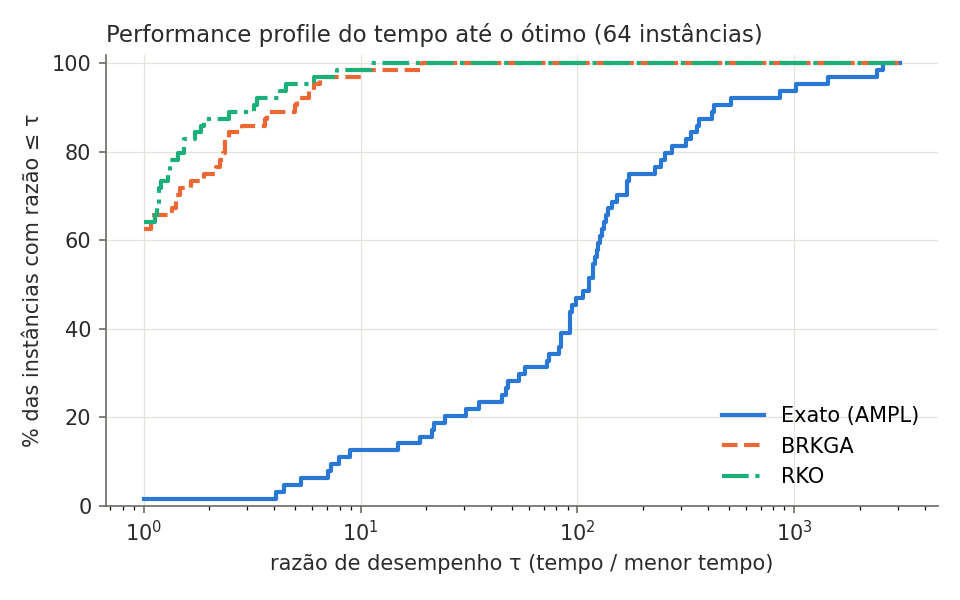
\includegraphics[width=0.49\textwidth]{../../resultados/figuras/perf_profile.png}\hfill
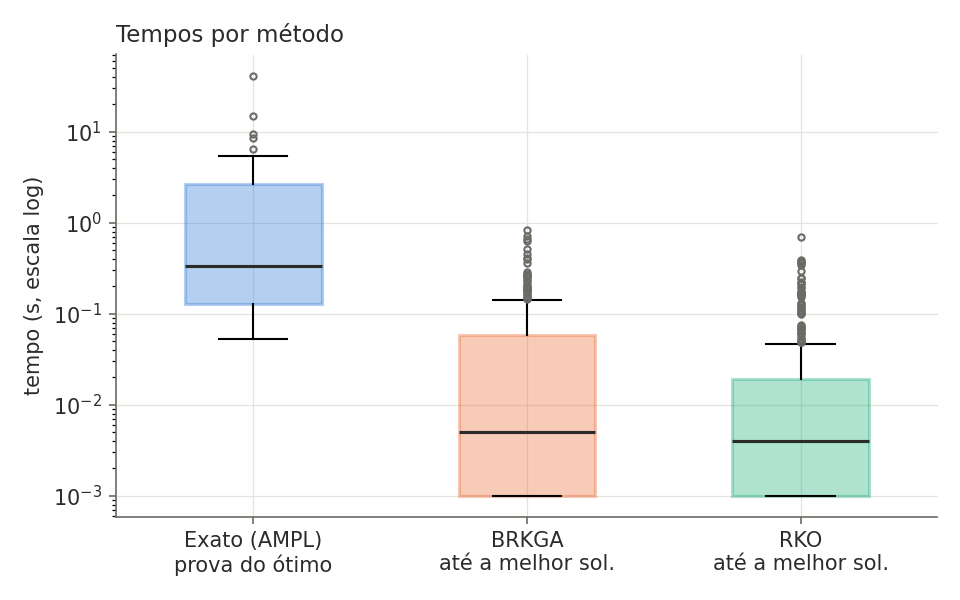
\includegraphics[width=0.49\textwidth]{../../resultados/figuras/boxplot_tempos.png}
\caption{Esquerda: performance profile (Dolan e Moré, 2002) do tempo até o ótimo. Direita: tempos por método.
\textbf{Atenção:} o exato mede o tempo até \emph{provar} o ótimo; as metaheurísticas, o tempo até
\emph{achar} o ótimo. Tempos abaixo de 1\,ms aparecem em $10^{-3}$.}
\end{figure}
\begin{figure}[H]
\centering
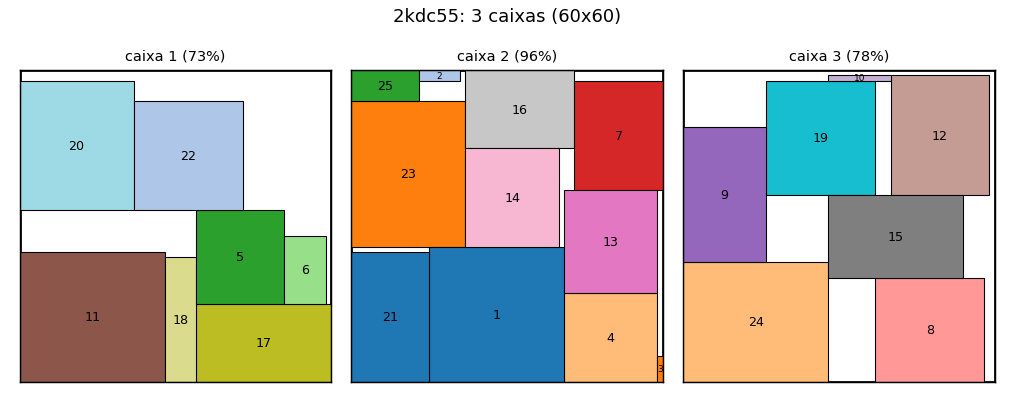
\includegraphics[width=0.9\textwidth]{../../resultados/figuras/2kdc55_ampl.png}
\caption{Gráfico qualitativo: solução ótima da instância 55 (3 caixas). A caixa 2 tem 96\% de ocupação,
o que explica a dificuldade de provar que não existe solução com menos caixas.}
\end{figure}

% =====================================================================
\section{Perguntas para o professor}\label{sec:atencao}
% =====================================================================
\newcommand{\resposta}{\par\noindent\textit{Resposta do professor:}\par
  \vspace{2pt}\noindent\rule{\linewidth}{0.3pt}\par\vspace{9pt}\noindent\rule{\linewidth}{0.3pt}\par
  \vspace{9pt}\noindent\rule{\linewidth}{0.3pt}\par\medskip}
\newcommand{\respostacurta}{\par\noindent{\color{cinza}\textit{Resposta:}}\ {\color{cinza!60}\hrulefill}\par\smallskip}
\newcommand{\principal}[2]{\par\medskip\Needspace{12\baselineskip}\noindent\atp{#1}\ \textbf{\large #2}\par\smallskip}
\newcommand{\secundaria}[2]{\par\smallskip\noindent\ats{#1}\ {\color{cinza}\textbf{#2}}\par}

\subsection{Principais}

\principal{1}{Os dois métodos resolvem as 64 instâncias muito rápido. Devemos usar instâncias sintéticas maiores ou deixar o problema mais difícil?}
\textbf{Contexto.} O exato prova os 64 ótimos em 150\,s no total (pior caso: 41\,s). O BRKGA acha o ótimo em
100\% das execuções, em 0,05\,s em média. Assim, a comparação exato $\times$ metaheurística diz pouco: os dois
``ganham'' sempre.\\
\textbf{Opções.} (a) Manter só as 64 da literatura. (b) Gerar instâncias \textbf{sintéticas maiores}
($n=50$, $100$) pelo mesmo procedimento das originais (tipos I--IV, densidades 7--16\%), onde o exato deve
estourar 3600\,s e a metaheurística passa a ser necessária. (c) Deixar o \textbf{problema} mais difícil (ex.:
permitir rotação, caixas de tamanhos diferentes): muda o modelo já escrito no artigo.\\
\textbf{Inclinação.} (b): criar \textbf{16 instâncias novas}, maiores, no mesmo formato das 64 (arquivos de dados
de entrada). Por exemplo: 4 tipos (I--IV) $\times$ 2 tamanhos ($n=50$ e $n=100$ itens) $\times$ 2 densidades de
conflito (7\% e 16\%). As 64 da literatura continuam sendo a base do artigo; as novas servem para ver os métodos
em casos onde o exato não resolve tudo rápido.
\resposta

\principal{2}{É isso que o senhor espera da parte de metaheurísticas?}
\textbf{Contexto.} Foi usado o RKO v2.0.1 com um decodificador próprio (Fig.~\ref{fig:dec}): as chaves dão a ordem dos
itens; cada item vai para a primeira caixa sem conflito onde cabe (Bottom-Left); a nota é o nº de caixas mais um
desempate. Toda solução é viável. O BRKGA do RKO sozinho foi comparado com o RKO completo (10 metaheurísticas), e
foram testadas 12 variantes do decodificador.\\
\textbf{Números.} BRKGA: 100\% das execuções no ótimo, 0,05\,s até a melhor solução. RKO: 99,7\%, 0,03\,s.\\
\textbf{Opções.} (a) Manter assim (BRKGA $\times$ RKO). (b) Comparar também as outras metaheurísticas do RKO
sozinhas (SA, ILS, VNS, \dots), todas com o mesmo decodificador; é barato, muda só a configuração.
(c) Investir em outra representação ou decodificador.\\
\textbf{Inclinação.} (a) + (b): atende ao ``comparar metaheurísticas diferentes'' pedido em aula.
\resposta

\principal{3}{O que fazer nas instâncias em que o LB não é atingível?}
\textbf{Contexto.} A metaheurística só sabe que achou o ótimo quando o nº de caixas é igual ao LB. Em
\textbf{32 das 64} instâncias o ótimo é maior que o LB (em 25 por 1 caixa, em 7 por 2; quase todas dos tipos I e
II). Nelas, a metaheurística acha o ótimo cedo, mas não consegue provar e segue até o tempo limite. Além disso,
com limite de tempo de relógio, o resultado mudou com a carga da máquina (quadro de correção, Seção 5.2).\\
\textbf{Opções.} (a) Parar por tempo e avaliar pelo \emph{gap} até o ótimo do exato, como a literatura faz com a
melhor solução conhecida. (b) Parar por \textbf{estagnação}: N avaliações do decodificador sem melhora, como em
Hammami, Rekik e Coelho (2020, \emph{Comput.\ Oper.\ Res.}\ 123); não depende da máquina. (c) Usar um
\textbf{LB mais forte} (o de Carlier et al., 2007, usado no artigo-base), para mais instâncias pararem cedo.\\
\textbf{Inclinação.} (b) + (c), avaliando sempre pelo gap até o ótimo do exato.
\resposta

\Needspace{24\baselineskip}
\begin{center}
\fcolorbox{cinza}{cinza!6}{\begin{minipage}{0.95\textwidth}\small
\textbf{Antes da pergunta: o que é o laço de cortes.} O modelo exato precisa de uma restrição (5) para
\emph{cada} grupo de itens que não cabe numa caixa. Com 25 itens existem $2^{25}\approx 33$ milhões de grupos:
não dá para escrever todas. O laço contorna isso (Fig.~\ref{fig:laco}):
\begin{enumerate}[leftmargin=*,itemsep=0pt,topsep=2pt]
\item resolve o modelo \textbf{sem} essas restrições (o ``mestre''): ele distribui os itens nas caixas respeitando
  área e conflitos, mas sem conferir se a arrumação geométrica é possível;
\item para cada caixa, confere com um segundo modelo exato (o 2D-OPP) se aqueles itens realmente cabem;
\item se um grupo não cabe, acrescenta uma restrição proibindo esse grupo (um \textbf{corte}) e volta ao passo 1;
\item quando todas as caixas cabem, a solução é \textbf{ótima}: o mestre já era o melhor possível mesmo com menos
  restrições.
\end{enumerate}
Na instância 53, por exemplo, foram 41 rodadas e 69 cortes até provar que o ótimo é 4 caixas.
\textbf{Por que perguntar:} no artigo-base (C++ com CPLEX), os cortes entram \emph{durante} uma única resolução
(``\emph{lazy constraints}'', via \emph{callbacks}). O AMPL não tem esse recurso, então o laço é um script que chama
o solver várias vezes. O método é o mesmo; só não é um único \texttt{solve}.
\end{minipage}}
\end{center}
\principal{4}{O laço de cortes em script AMPL é aceito como ``método exato''?}
\textbf{Contexto.} O AMPL não tem \emph{callbacks}: o mestre é resolvido várias vezes, ganhando os cortes (5)
de grupos que não cabem (Fig.~\ref{fig:laco}). Se não for aceito, a Etapa 5 muda.\\
\textbf{Números.} 64/64 ótimos provados, 150\,s no total; todos os 780 cortes conferidos por outro método exato
(CP-SAT).\\
\textbf{Inclinação.} Aceitar como está.
\resposta

\subsection{Secundárias (podem ficar para depois)}
{\color{cinza}\small
\secundaria{1}{$n$ chaves (só a ordem) ou $2n$ (ordem + regra de escolha por item)?}
$2n$ não melhorou nenhuma instância e dobra o espaço de busca. \emph{Inclinação:} $n$ chaves.
\respostacurta
\secundaria{2}{O desempate (área da caixa mais vazia $\div WH$) é adequado?}
Na 48: 0--20\% de acerto sem desempate, 60--100\% com. \emph{Inclinação:} manter; testar outro se sugerido.
\respostacurta
\secundaria{3}{A forma de semear as threads do RKO está correta?}
No \texttt{main.cpp} original, \texttt{private(rng)} dá a cada thread a semente padrão. O \texttt{main} adaptado
semeia cada thread. \emph{Inclinação:} manter e avisar os mantenedores.
\respostacurta
\secundaria{4}{Quantas execuções por instância e quais métricas?}
Aula: $\sim$100 sementes; Hammami et al.: 20 execuções (nº de ótimos, gap, melhor/média, estabilidade, tempo
até a melhor). \emph{Inclinação:} 100 execuções + essas métricas + performance profile + Wilcoxon/Friedman.
\respostacurta
\secundaria{5}{É justo comparar o RKO (10 threads, Q-Learning) com o BRKGA (1 thread, parâmetros fixos)?}
O RKO acha a melhor solução $\sim$1,7$\times$ mais rápido, com 10$\times$ mais threads e outro modo de
parâmetros. \emph{Inclinação:} mesmo tempo de relógio, informando as threads, e o mesmo modo de parâmetros.
\respostacurta
\secundaria{6}{Podemos usar a 01 reconstruída e as 53--64 geradas?}
O \texttt{2kdc01} do zip é cópia da 02; as 53--64 não vieram. \emph{Inclinação:} usar e declarar no artigo.
\respostacurta
\secundaria{7}{O IPR do RKO não confere a flag de parada: é intencional?}
Contorno adotado: o decodificador zera o \texttt{MAXTIME}. \emph{Inclinação:} manter e avisar os mantenedores.
\respostacurta
}

\subsection*{Sugestões (não são dúvidas)}
\begin{itemize}[leftmargin=*,itemsep=1pt]
\item Compactar os desenhos do AMPL para baixo e para a esquerda (hoje alguns itens ``flutuam''; é estético).
\item Soluções iniciais ``inteligentes'' (área ou grau decrescente): exigiriam mexer no código genérico do RKO; ganho esperado pequeno.
\end{itemize}

\subsection*{O que falta}
\begin{itemize}[leftmargin=*,itemsep=1pt]
\item Experimento final da metaheurística (depende de \atp{1}, \atp{3}, \ats{4} e \ats{5}).
\item Testes estatísticos (Wilcoxon/Friedman) e gráfico de convergência.
\item Seções 5--7 do artigo (resultados exatos, comparação, conclusão).
\end{itemize}

% =====================================================================
\section{Software, versões e de onde vieram}
% =====================================================================
\begin{center}\small
\begin{tabular}{@{}p{3.6cm}p{3.4cm}p{8.6cm}@{}}
\toprule
Componente & Versão & Origem / observação \\ \midrule
\textbf{RKO} (C++) & \textbf{2.0.1} (README) & \url{https://github.com/RKO-solver/RKO_Cpp_v2.0}, commit
  \texttt{126e358} (14/03/2026), clonado em 09/11/2026 em \texttt{meta/RKO\_Cpp\_v2.0}. Chaves et al. (2025),
  \emph{J.\ Heuristics} 31(4). O BRKGA usado é o do próprio RKO (\texttt{MH/BRKGA.h}) \\
AMPL & 20261109 & via \texttt{amplpy} 0.18.0 (PyPI); licença demo do pacote --- suficiente para as 64 instâncias \\
HiGHS & 1.15.1 & solver gratuito, módulo do amplpy (\texttt{amplpy.modules install highs}) \\
OR-Tools (CP-SAT) & 9.15.6755 & PyPI; só para auditar os cortes \\
Python & 3.10.12 & numpy 2.2.6, pandas 2.3.3, networkx 3.4.2, matplotlib 3.10.9 \\
g++ / OpenMP & 11.4.0 & \texttt{-O3 -march=native -fopenmp -std=c++20} \\
Máquina & --- & Intel Core i5-13420H (12 threads), 23\,GB de RAM, Linux \\
Instâncias & --- & \texttt{2bppc.zip} do site do Hokama (52 arquivos) + 13 reconstruídas/geradas \\
\bottomrule
\end{tabular}
\end{center}

% =====================================================================
\section{Glossário rápido}
% =====================================================================
{\small
\begin{description}[leftmargin=*,itemsep=0pt,font=\normalfont\bfseries]
\item[LB / UB] limitante inferior (não dá para usar menos caixas) / superior (uma solução que já temos).
\item[2D-OPP] problema de decisão ``este grupo de retângulos cabe numa caixa?''; NP-difícil.
\item[Corte (5)] restrição que proíbe um grupo que não cabe de ficar junto em qualquer caixa.
\item[Instância] um arquivo de dados de entrada: itens, caixa e conflitos (ex.: \texttt{2kdc48}).
\item[Execução / semente] rodar a metaheurística uma vez numa instância; a semente inicia o gerador aleatório
  (mesma semente $\Rightarrow$ mesmo caminho de busca).
\item[Chave aleatória] número em $[0,1)$; um vetor de chaves representa uma solução via decodificador.
\item[FF / BF] \emph{First Fit} (primeira caixa que serve) / \emph{Best Fit} (a mais cheia que serve).
\item[Maximal Rectangles] guarda os retângulos livres máximos da caixa; o item vai num deles.
\item[BL / BSSF] \emph{Bottom-Left} (posição mais baixa, depois mais à esquerda) / \emph{Best Short Side Fit}
  (menor sobra no lado curto).
\item[Pool de elite] as 10 melhores soluções do RKO, compartilhadas entre as metaheurísticas.
\item[Thread / núcleo] thread é uma linha de execução; ela roda num núcleo do processador. Esta máquina tem 4
  núcleos rápidos (2 threads cada) e 4 lentos: 12 threads ao todo.
\item[Q-Learning] modo do RKO que ajusta os parâmetros das metaheurísticas durante a busca.
\item[Performance profile] curva com a fração das instâncias em que cada método está a até
  $\tau\times$ do melhor tempo.
\end{description}}

\end{document}
